\subsection*{Aufgabe 17}
Gegeben ist die Dispersionsrelation für ein fcc-Gitter:
\begin{align}
\label{eq-disp}
  E(k) = E'_\alpha - 4\;|A| \left(\cos\frac{k_x a}{2}\cos\frac{k_y a}{2} +
    \cos\frac{k_y a}{2}\cos\frac{k_z a}{2} + \cos\frac{k_z a}{2}\cos\frac{k_x a}{2} \right)
\end{align}

\subsubsection*{a)}
\begin{wrapfigure}[11]{R}{8cm}
  \centering
  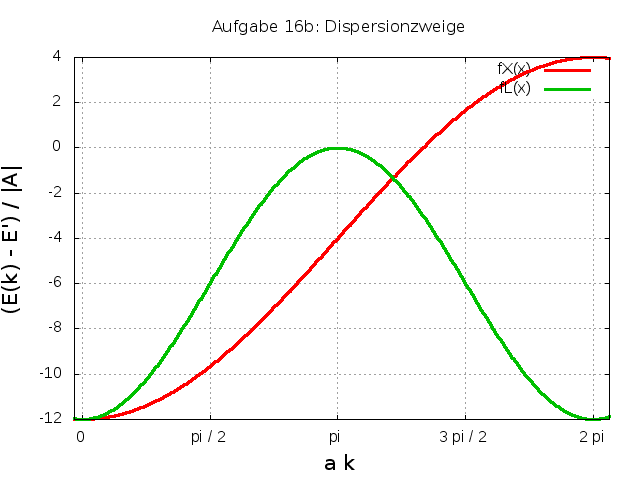
\includegraphics[width=7.5cm]{aufgabe16b.png}
\label{bild16b}
\end{wrapfigure}
Im LCAO-Modell beschreibt das Austauschintegral A den Overlap der Wellenfunktion
eines (Valenz-)Elektrons mit den Wellenfunktionen der Elektronen benachbarter Atome.
Die daraus resultierende Aufspaltung der Bänder ist propotional zu A und einem
Geometriefaktor (runde Klammer in obiger Formel) und ist dadurch auch abhängig
von $\vec k$.
\newline
\subsubsection*{b)}
\begin{itemize}
\item[$\Gamma$ X:]
  In $\Gamma$X-Richtung ist $k_y = k_z = 0$, sei $k:= k_x$, dann wird \eqref{eq-disp}
  wegen $\cos(0) = 1$:
\begin{align*}
    E(k) = E'_\alpha - 4\;|A| \left(1 + 2 \cos\frac{k a}{2} \right)
\end{align*}
Siehe rote Kurve fX im Plot. Da $\cos(k)$ Werte zwischen -1 und +1 annehmen kann
ergibt sich eine Bandbreite $B = 16\;|A|$.
\item[$\Gamma$ L:]
  In $\Gamma$L-Richtung ist $k_x = k_y = k_z =: k$, dann wird \eqref{eq-disp}:
\begin{align*}
    E(k) = E'_\alpha - 4\;|A| \left(3 \cos^2\frac{k a}{2} \right)
\end{align*}
Siehe grüne Kurve fL im Plot. Da $\cos^2(k)$ Werte zwischen 0 und +1 annehmen kann
ergibt sich eine Bandbreite $B = 12\;|A|$.
\end{itemize}

\subsubsection*{c)}
% Blindtext
Weit hinten, hinter den Wortbergen, fern der Länder Vokalien und Konsonantien leben die Blindtexte. Abgeschieden wohnen Sie in Buchstabhausen an der Küste des Semantik, eines großen Sprachozeans. Ein kleines Bächlein namens Duden fließt durch ihren Ort und versorgt sie mit den nötigen Regelialien. Es ist ein paradiesmatisches Land, in dem einem gebratene Satzteile in den Mund fliegen. Nicht einmal von der allmächtigen Interpunktion werden die Blindtexte beherrscht – ein geradezu unorthographisches Leben.

Eines Tages aber beschloß eine kleine Zeile Blindtext, ihr Name war Lorem Ipsum, hinaus zu gehen in die weite Grammatik. Der große Oxmox riet ihr davon ab, da es dort wimmele von bösen Kommata, wilden Fragezeichen und hinterhältigen Semikoli, doch das Blindtextchen ließ sich nicht beirren. Es packte seine sieben Versalien, schob sich sein Initial in den Gürtel und machte sich auf den Weg.

Als es die ersten Hügel des Kursivgebirges erklommen hatte, warf es einen letzten Blick zurück auf die Skyline seiner Heimatstadt Buchstabhausen, die Headline von Alphabetdorf und die Subline seiner eigenen Straße, der Zeilengasse. Wehmütig lief ihm eine rethorische Frage über die Wange, dann setzte es seinen Weg fort.

Unterwegs traf es eine Copy. Die Copy warnte das Blindtextchen, da, wo sie herkäme wäre sie zigmal umgeschrieben worden und alles, was von ihrem Ursprung noch übrig wäre, sei das Wort "und" und das Blindtextchen solle umkehren und wieder in sein eigenes, sicheres Land zurückkehren.

Doch alles Gutzureden konnte es nicht überzeugen und so dauerte es nicht lange, bis ihm ein paar heimtückische Werbetexter auflauerten, es mit Longe und Parole betrunken machten und es dann in ihre Agentur schleppten, wo sie es für ihre Projekte wieder und wieder mißbrauchten. Und wenn es nicht umgeschrieben wurde, dann benutzen Sie es immernoch.
